\documentclass[11pt]{beamer}

\usetheme{metropolis}

\usepackage{graphicx}
\usepackage{physics}
\usepackage{adjustbox}
\usepackage{caption}
\usepackage{chemformula}
\usepackage{quoting}
\usepackage[style=chem-angew,backend=bibtex]{biblatex}
\bibliography{references}
%
% Choose how your presentation looks.
%
% For more themes, color themes and font themes, see:
% http://deic.uab.es/~iblanes/beamer_gallery/index_by_theme.html
%
\mode<presentation>
{
  \usetheme{default}      % or try Darmstadt, Madrid, Warsaw, ...
  \usecolortheme{default} % or try albatross, beaver, crane, ...
  \usefonttheme{default}  % or try serif, structurebold, ...
  \setbeamertemplate{navigation symbols}{}
  \setbeamertemplate{caption}[numbered]
  \setbeamerfont{footnote}{size=\tiny}
} 

\usepackage[english]{babel}
\usepackage[utf8]{inputenc}
\graphicspath{{image/}}

\AtBeginSection[]{
\begin{frame}{Outline}
  \tableofcontents[currentsection]
\end{frame}
}

\title{Chapter 6: Quantities in Chemical Reactions}
\institute{Chemistry Department, Cypress College}
\date{October 3, 2022}

\begin{document}

\begin{frame}
  \titlepage
\end{frame}

\begin{frame}{Class Annoucements}
  \textbf{Lab}
  \begin{itemize}
  \item Double Displacement Reactions - precipitation rules
    and acid base reactions
  \item Use 1mL of each solution
  \item Recall indications for chemical reaction (color, solids,
    temp, etc.)
  \end{itemize}
  
  \textbf{Lecture}
  \begin{itemize}
  \item Keep submitting the homework assignment on time
    ($\sim 1-2$ hours grace period)
  \item Go over homework 4 - present and get 1 EC point
  \item Quiz submissions are slacking (Quiz 5 due tonight
    at 11:59pm)
  \item Homework and Quiz will be released Fri, Oct 7 at 3pm
  \end{itemize}
\end{frame}

\section{Stoichiometry: Relationship Between Reactants and Products}

\begin{frame}{Balanced Chemical Equation: Photosynthesis}
  \centering
  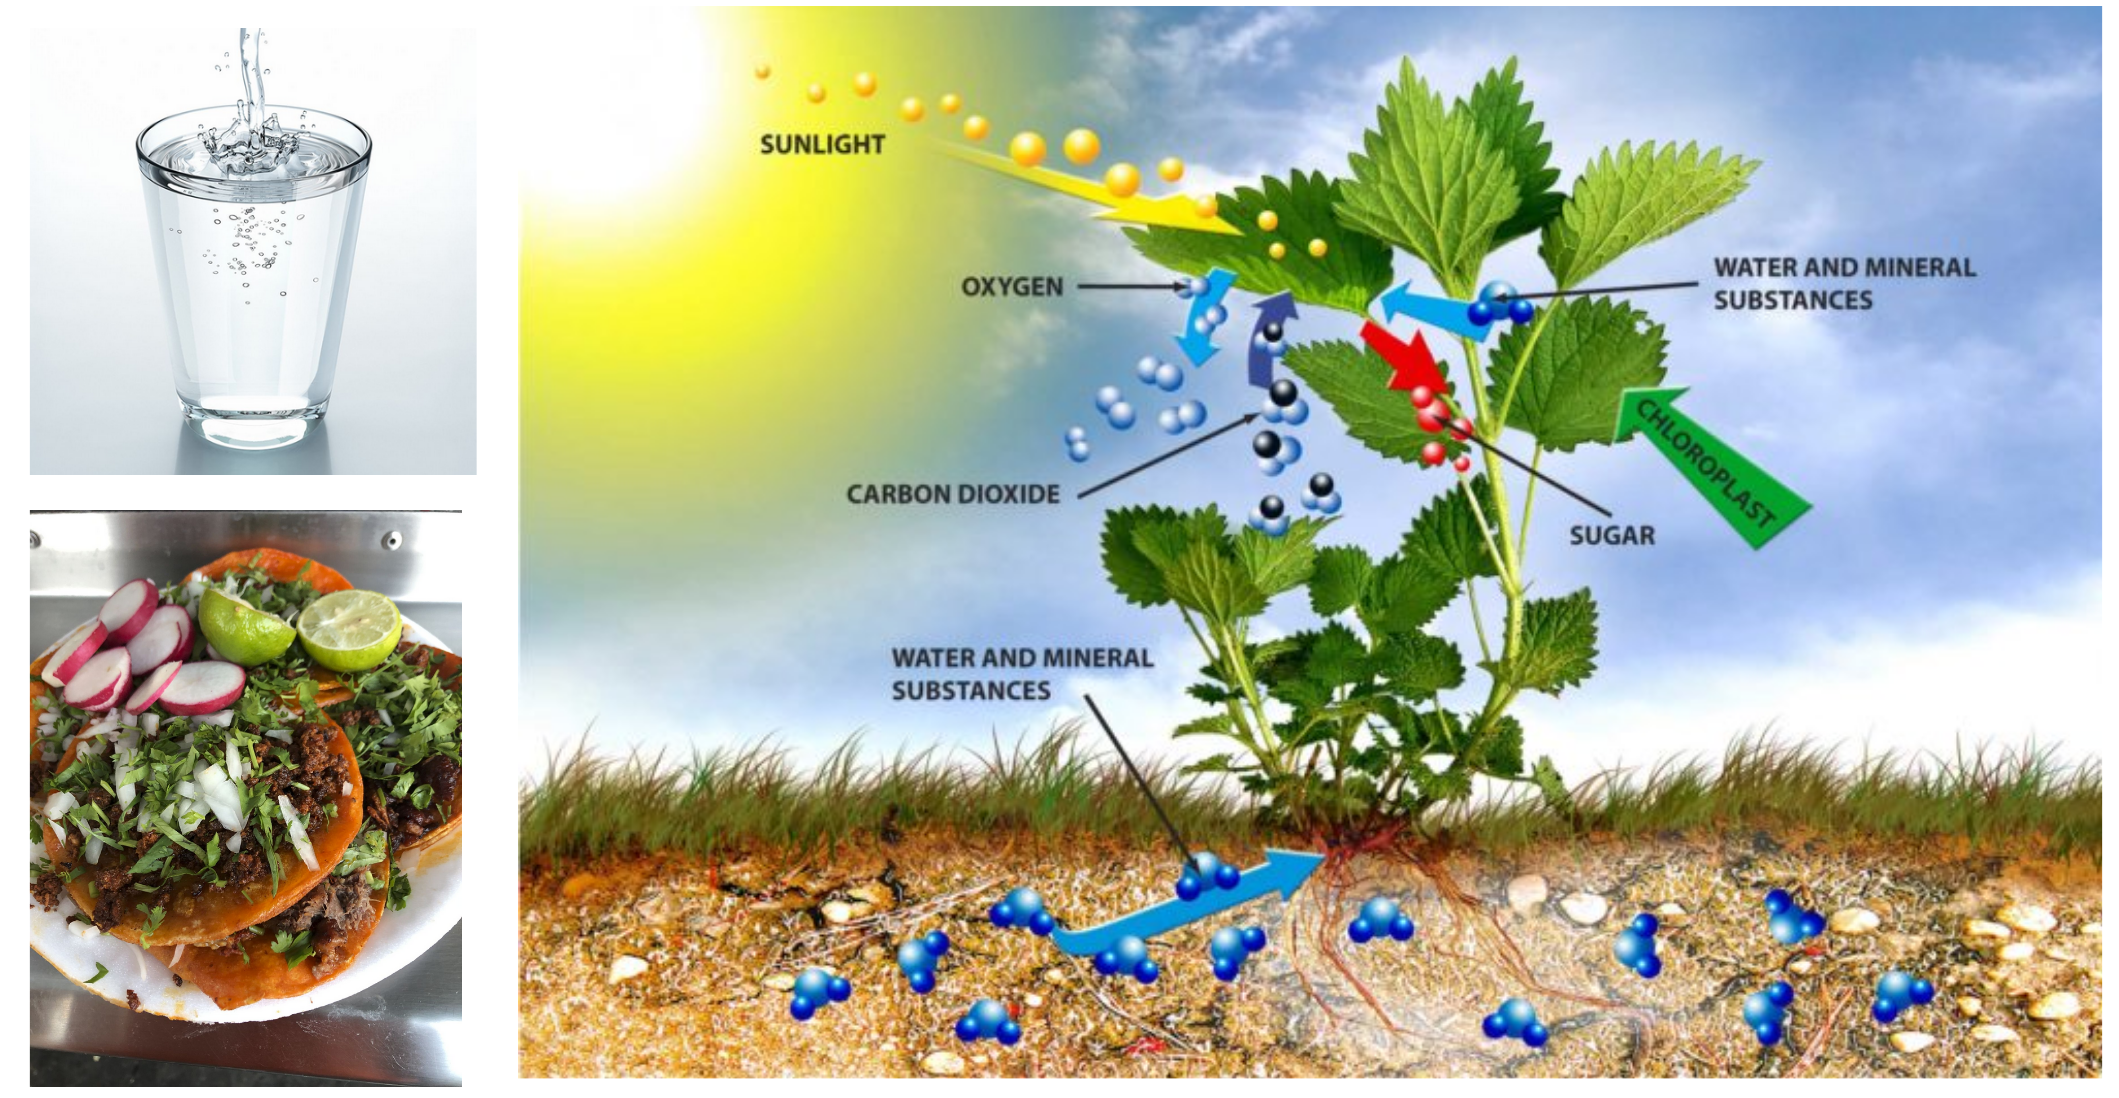
\includegraphics[trim={8in 0 0 0},clip,width=1\linewidth]{food_pic}
\end{frame}

\begin{frame}{Meaning of a Balanced Equation}
  \textbf{Photosysnthesis Chemical Equation}
  \begin{equation}
    6\text{CO$_2$(g)} + 6\text{H$_2$O(l)} \rightarrow \text{C$_6$H$_{12}$O$_6$(s)}
    + 6\text{O$_2$(g)}
  \end{equation}
  
  \begin{itemize}
  \item Balanced chemical equation satisfies the conservation of mass
  \item Coefficients in front of the molecules represent the relative
    moles of reactants and products
  \item Hence, moles of reactants and products are not necessarily
    equal
  \end{itemize}
\end{frame}

\begin{frame}{What can be accomplished with a balanced equation?}
  \begin{center}
    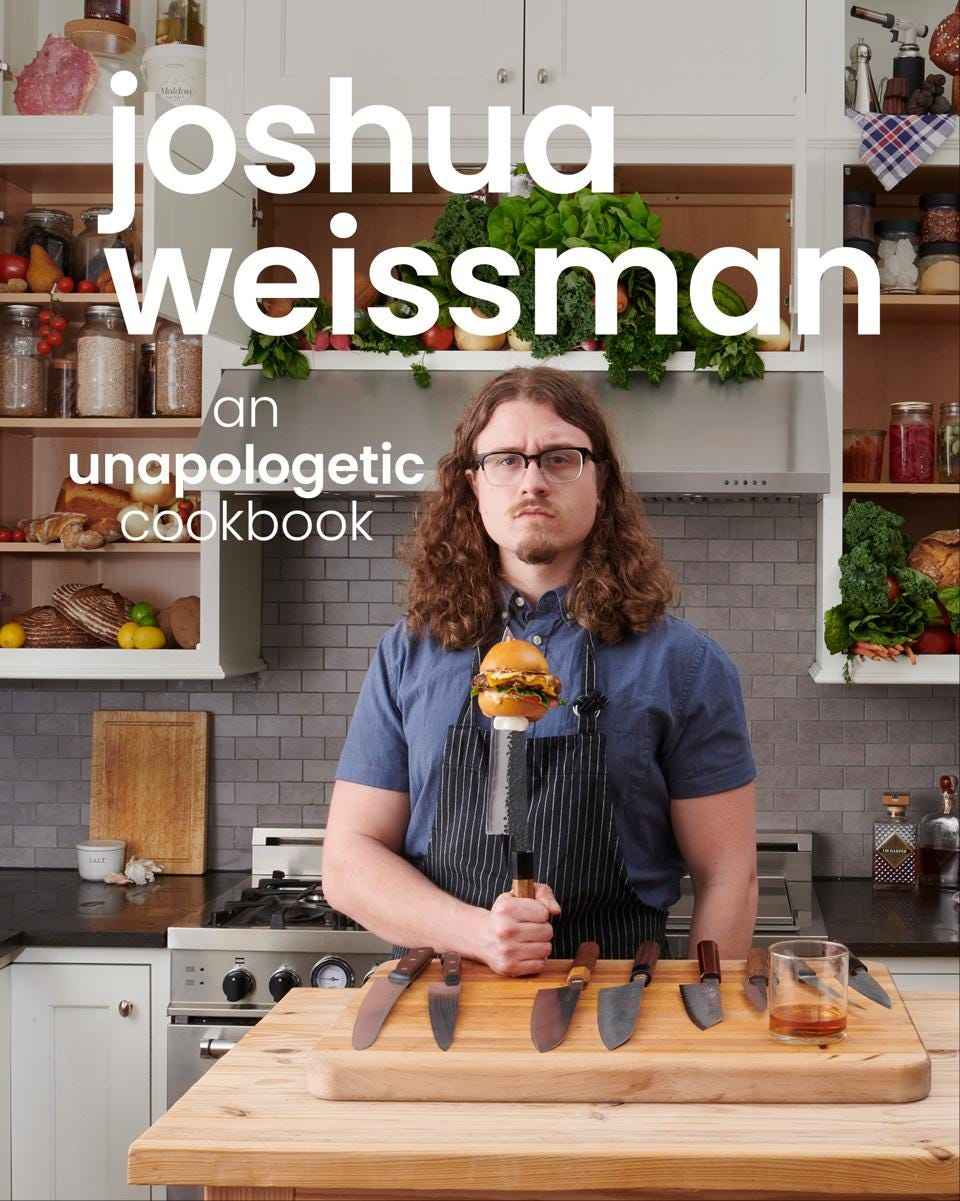
\includegraphics[scale=0.11]{josh_weiss}
  \end{center}
  
  \begin{itemize}
  \item Analogy: \href{https://www.youtube.com/watch?v=T5SYu8tyKjM}{Cookbook recipe-
    Popeyes Chicken but better}
  \item Provides the means to determine how much product is
    produced for a given amount of reactants
  \item Relate to molar masses, number of molecules, amount
    of moles and masses
  \end{itemize}  
\end{frame}

\subsection{Mole-mole Conversion}

\begin{frame}{Example: Mole-mole Conversion}
  If 1.14 mol of CO$_2$(g) was formed by combustion of C$_3$H$_8$(g),
  how many moles of H$_2$O(g) were also formed?

  \textbf{Determine:} What is given and what is the question asking?

  \onslide<2->{Given: 1.14 mol CO$_2$ formed; Question: amount of H$_2$O in
    mols}

  \onslide<3->{C$_3$H$_8$(g) + 5O$_2$(g) $\rightarrow$ 3CO$_2$(g) + 4H$_2$O(g)}
  \onslide<4->{
    \begin{align*}
      1.14 \text{mol CO$_2$} \times \frac{4\text{mol H$_2$O}}{3\text{mol CO$_2$}} = 1.52\text{mol H$_2$O}
    \end{align*}
  }
\end{frame}

\begin{frame}{Example: Mole-mole Conversion}
  Pure methanol (CH$_3$OH) is used as a fuel for race cars in the Indy Racing Leauge
  and in the Championship Auto Racing Teams. Given that 1.00 gal of methanol
  contains 94.5 mol, how many moles of oxygen will react with 1.00 gal of
  methanol?

  \textbf{Determine:} What is given and what is the question asking?
  
  \onslide<2->{Given 94.5 mol CH$_3$OH; Question: amount of mols O$_2$ required}

  \onslide<3->{CH$_3$OH(l) + O$_2$(g) $\rightarrow$ CO$_2$(g) + H$_2$O(g)
    \begin{align*}
      94.5 \text{mol CH$_3$OH} \times \frac{3\text{mol O$_2$}}{2 \text{molCH$_3$OH}}
        = 142 \text{mol O$_2$}
    \end{align*}
  }
\end{frame}

\subsection{Mass-mass Conversion}

\begin{frame}{Example: Mass-mass Conversion}
  Suppose we have 9.20g Na(s). How many grams of Cl$_2$(g) should
  react with this amount of Na(s)?

  \textbf{Determine:} What is given and what is the question asking?

  \onslide<2->{Given: 9.20g Na; Question: amount of Cl$_2$ in g needed

  \textbf{Q:} What is the quantity needed to convert between mols and grams?}

\end{frame}

\end{document}
